\subsection{Life cycle of a Particle object}

A Particle is created by the EarthView ShowOff module when a Story comes in.
The object gets a lifetime based on the publication date of the story (as was
specified in the document it originated from, e.g. the RSS feed). Initially,
its state will be `new', after which it is launched and gets into state
`launch'.

The particle will reach a set height and when it reaches this, the state
changes into `orbit'. It will now assume a circular orbit around the center.

While the particle exists, it can also receive Analysis messages for the Story
it represents. These Analyses influence the orbit of the particle, but only
when its state is `orbit'.

After some time, for instance two days, the article is considered old and
the particle's lifetime is over. It will get into state `crashing' to
indicate that it is leaving its orbit towards the center, spiraling in
until it reaches a certain height. When it reaches this, its state will
become `crashed' and that is an indication that the particle can be safely
removed from the system.

\begin{figure}
  \centering
  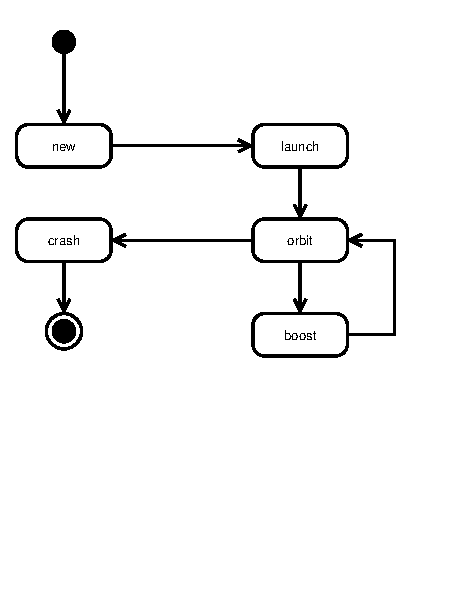
\includegraphics{image/sequence-diagram-particle}
  \caption{The life cycle model of a Particle object}
\end{figure}
